\documentclass[aspectratio=169]{beamer}
\usepackage{fontspec}
\usepackage{polyglossia}
\usepackage{color}
\usepackage{listings}
\setdefaultlanguage{russian}
\usepackage{csquotes}
\usetheme{metropolis}
\metroset{background=light}
\metroset{sectionpage=none}
\metroset{numbering=fraction}

\definecolor{ssaublue}{RGB}{77,144,205}
\setbeamercolor{frametitle}{fg=white, bg=ssaublue}
\setbeamercolor{title separator}{fg=ssaublue}

\setmainfont[
    Path = ../fonts/elektratextpro/,
    Extension = .otf,
    UprightFont = elektratextpro,
    BoldFont = elektratextpro_bold,
    ItalicFont = elektratextpro_italic,
    BoldItalicFont = elektratextpro_bolditalic
]{elektratextpro}

\setsansfont[
    Path = ../fonts/elektratextpro/,
    Extension = .otf,
    UprightFont = elektratextpro,
    BoldFont = elektratextpro_bold,
    ItalicFont = elektratextpro_italic,
    BoldItalicFont = elektratextpro_bolditalic
]{elektratextpro}

\setmonofont[
    Path = ../fonts/elektratextpro/,
    Extension = .otf,
    UprightFont = elektratextpro,
    BoldFont = elektratextpro_bold,
    ItalicFont = elektratextpro_italic,
    BoldItalicFont = elektratextpro_bolditalic
]{elektratextpro}

\newfontfamily\cyrillicfont[
    Path = ../fonts/elektratextpro/,
    Extension = .otf,
    UprightFont = elektratextpro,
    BoldFont = elektratextpro_bold,
    ItalicFont = elektratextpro_italic,
    BoldItalicFont = elektratextpro_bolditalic
]{elektratextpro}

\newfontfamily\cyrillicfontsf[
    Path = ../fonts/elektratextpro/,
    Extension = .otf,
    UprightFont = elektratextpro,
    BoldFont = elektratextpro_bold,
    ItalicFont = elektratextpro_italic,
    BoldItalicFont = elektratextpro_bolditalic
]{elektratextpro}

\newfontfamily\cyrillicfonttt[
    Path = ../fonts/elektratextpro/,
    Extension = .otf,
    UprightFont = elektratextpro,
    BoldFont = elektratextpro_bold,
    ItalicFont = elektratextpro_italic,
    BoldItalicFont = elektratextpro_bolditalic
]{elektratextpro}

% Настройка листингов для Beamer
\lstset{
    basicstyle=\ttfamily\footnotesize,
    commentstyle=\color{gray},
    columns=fullflexible,
    keepspaces=true,
    breaklines=false,
    extendedchars=true,
    texcl=true,
    showstringspaces=false
}

\title{Docker: сеть, volumes, bind mounts}
\date{15 октября 2025 г.}

\begin{document}

\maketitle

\begin{frame}{Коммутатор (network switch)}
    \begin{center}
        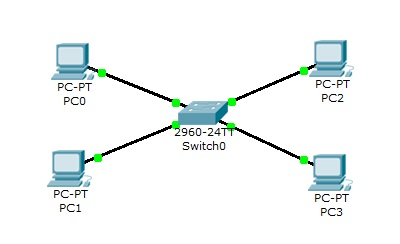
\includegraphics[width=0.6\textwidth]{media/switch}
    \end{center}
\end{frame}

\begin{frame}{Сетевой мост (network bridge)}
    \begin{center}
        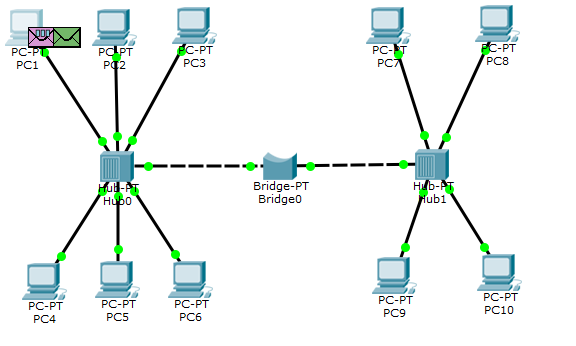
\includegraphics[width=0.6\textwidth]{media/net-bridge}
    \end{center}
\end{frame}

\begin{frame}{Linux bridge}
    \begin{center}
        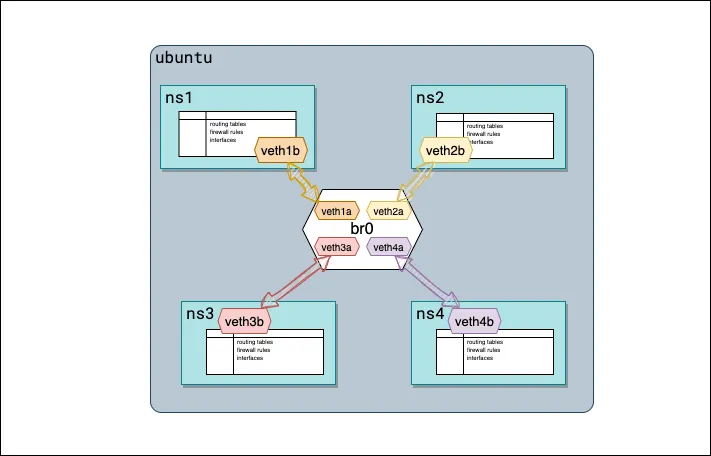
\includegraphics[width=0.6\textwidth]{media/bridge}
    \end{center}
    \footnotesize{\textcolor{gray}{\url{https://medium.com/@amazingandyyy/learn-linux-bridge-with-graphs-a425aa92945f}}}
\end{frame}

\begin{frame}{Демонстрация: Linux bridge}
    \textbf{Что покажем:}
    \begin{enumerate}
        \item Linux network namespaces
        \item Linux network bridge
    \end{enumerate}

    \vspace{0.2cm}

    \textbf{Демо-репозиторий:} \\
    \href{https://github.com/prafdin/devops-course-demos/tree/docker-additional}{\texttt{https://github.com/prafdin/devops-course-demos/tree/docker-additional}}
\end{frame}

\begin{frame}{Container Network Model}
    \begin{center}
        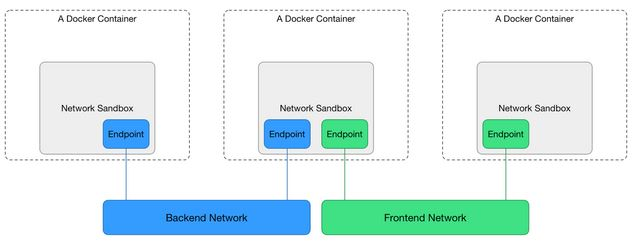
\includegraphics[width=0.6\textwidth]{media/cnm-model}
    \end{center}

    \footnotesize{\textcolor{gray}{\url{https://github.com/moby/libnetwork/blob/master/docs/design.md}}}
\end{frame}

\begin{frame}{Libnetwork}
    \begin{center}
        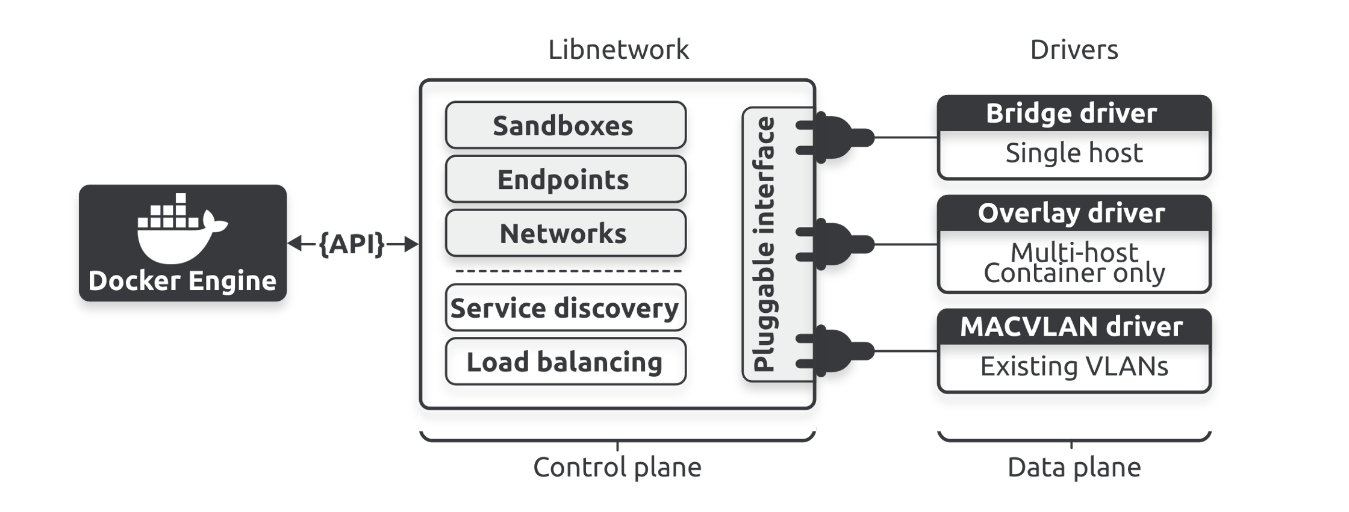
\includegraphics[width=0.75\textwidth]{media/libnetwork}
    \end{center}

    \footnotesize{\textcolor{gray}{\url{https://github.com/moby/moby/tree/28.x/libnetwork}}}
\end{frame}

\begin{frame}{Демонстрация: Docker network}
    \textbf{Что покажем:}
    \begin{enumerate}
        \item Команды docker network
    \end{enumerate}

    \vspace{0.2cm}

    \textbf{Демо-репозиторий:} \\
    \href{https://github.com/prafdin/devops-course-demos/tree/docker-additional}{\texttt{https://github.com/prafdin/devops-course-demos/tree/docker-additional}}
\end{frame}

\begin{frame}{SNAT}
    \begin{center}
        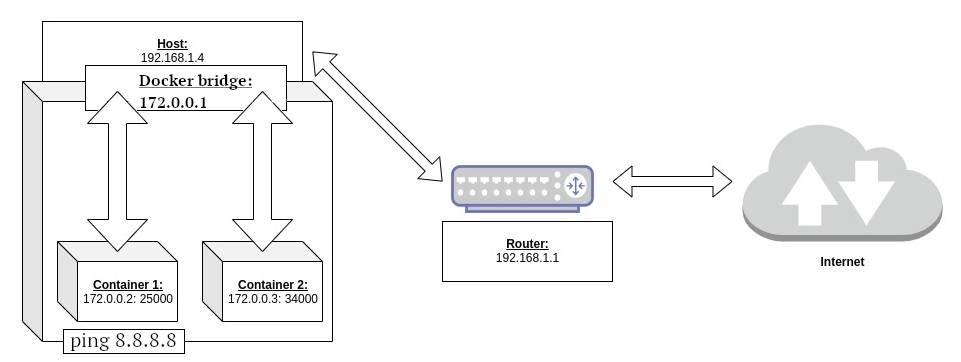
\includegraphics[width=1\textwidth]{media/cont-to-internet}
    \end{center}

    \footnotesize{\textcolor{gray}{\href{https://imehboob.medium.com/linux-networking-snat-and-packet-forwarding-to-connect-to-internet-from-namespace-part-4-558a505794bd}{https://imehboob.medium.com/linux-networking...}}}
\end{frame}

\begin{frame}{Port publishing (DNAT)}
    \begin{center}
        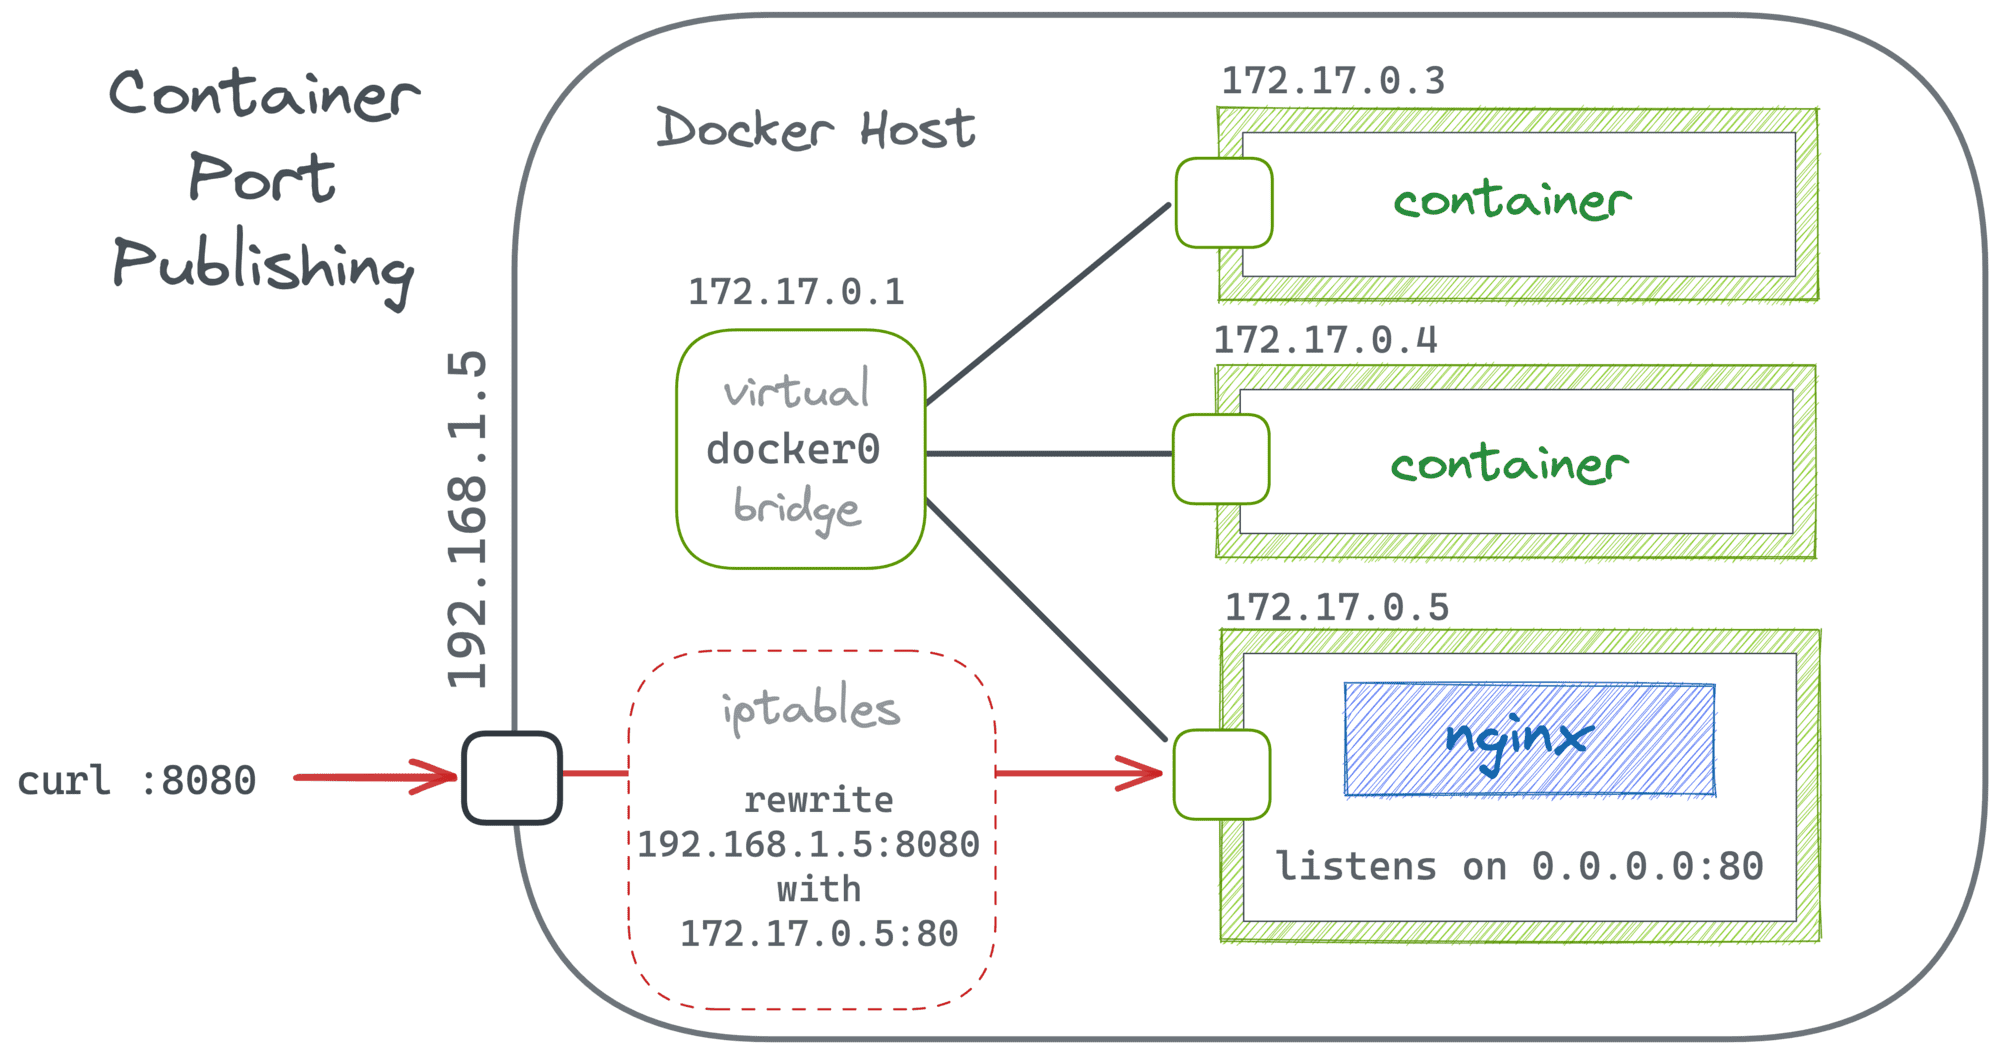
\includegraphics[width=0.8\textwidth]{media/to-cont}
    \end{center}

    \footnotesize{\textcolor{gray}{\url{https://iximiuz.com/en/posts/docker-publish-container-ports/}}}
\end{frame}

\begin{frame}{Демонстрация: docker и NAT}
    \textbf{Что покажем:}
    \begin{enumerate}
        \item Команды docker network
    \end{enumerate}

    \vspace{0.2cm}

    \textbf{Демо-репозиторий:} \\
    \href{https://github.com/prafdin/devops-course-demos/tree/docker-additional}{\texttt{https://github.com/prafdin/devops-course-demos/tree/docker-additional}}
\end{frame}

\begin{frame}{RW Layer}
    \begin{center}
        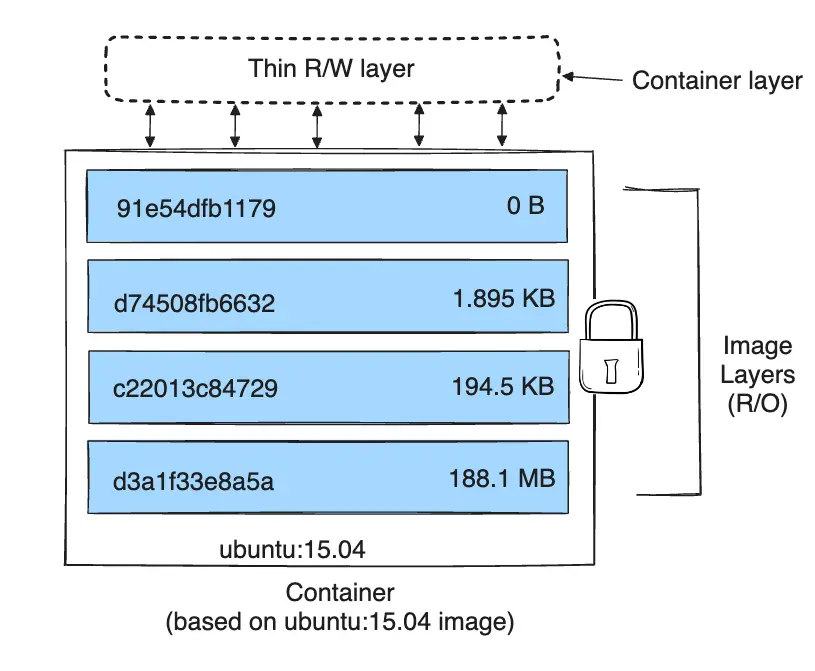
\includegraphics[width=0.5\textwidth]{media/container-layers}
    \end{center}
\end{frame}

\begin{frame}{Docker Storage}
    \begin{center}
        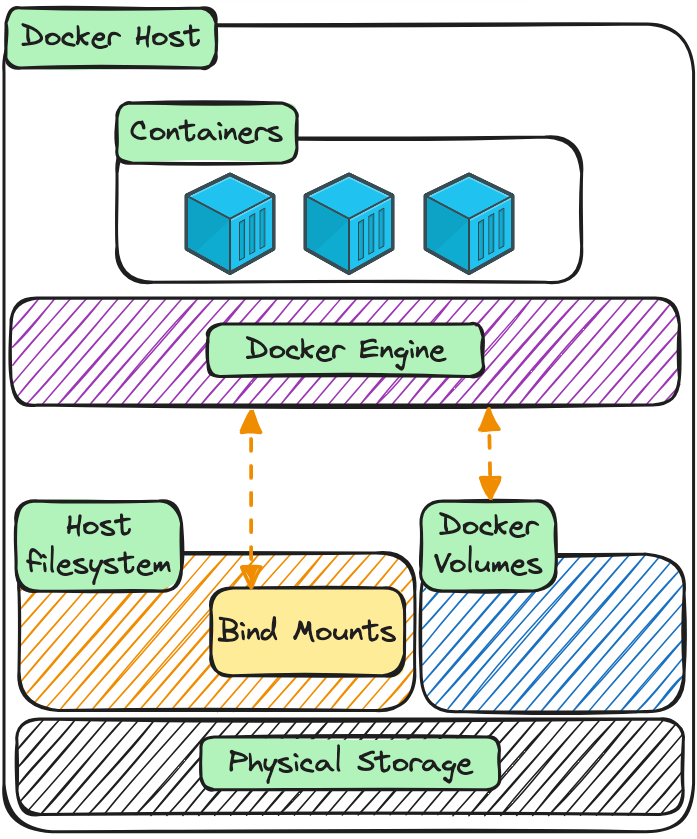
\includegraphics[width=0.40\textwidth]{media/docker-storage}
    \end{center}

    \footnotesize{\textcolor{gray}{\url{https://iamachs.com/blog/docker/part-5-understanding-docker-storage-and-volumes/}}}
\end{frame}

\begin{frame}{Docker Volume}
    \begin{center}
        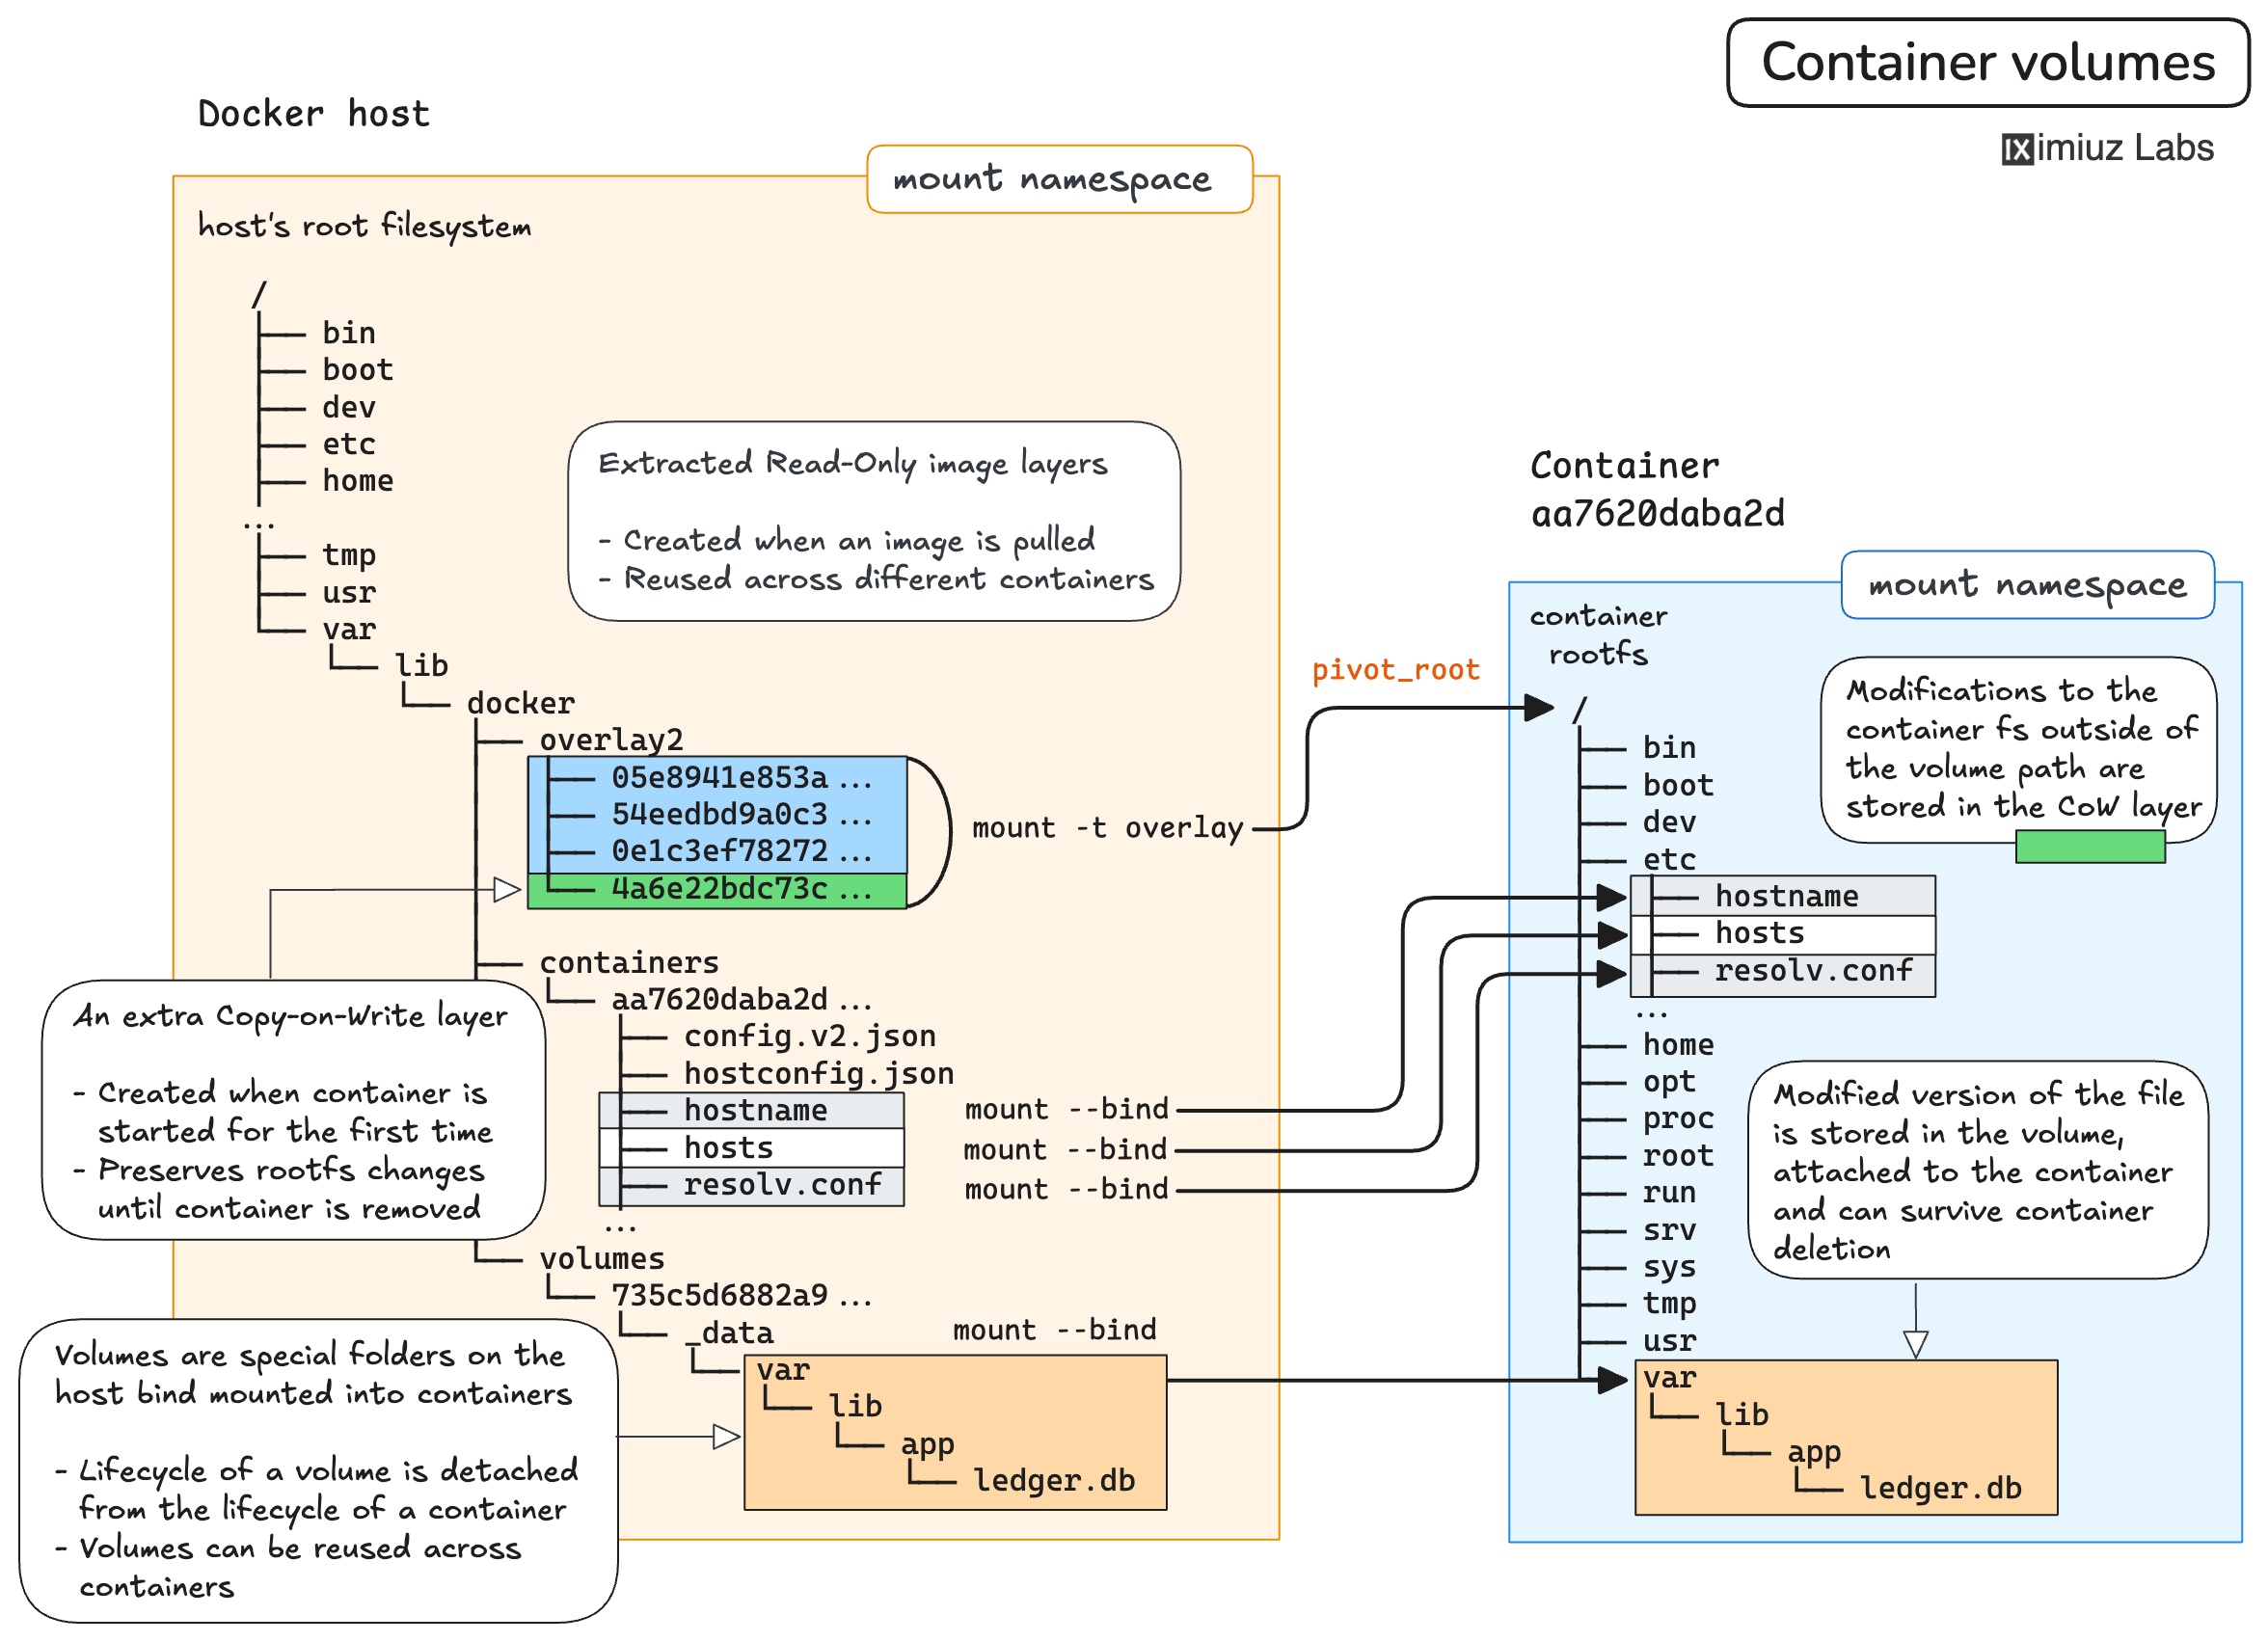
\includegraphics[width=0.62\textwidth]{media/container-volumes}
    \end{center}

    \footnotesize{\textcolor{gray}{\url{https://labs.iximiuz.com/tutorials/container-filesystem-from-scratch}}}
    \footnotesize{\textcolor{gray}{\url{https://docs.docker.com/engine/extend/legacy_plugins/\#volume-plugins}}}
\end{frame}

\begin{frame}{Bind Mount}
    \begin{center}
        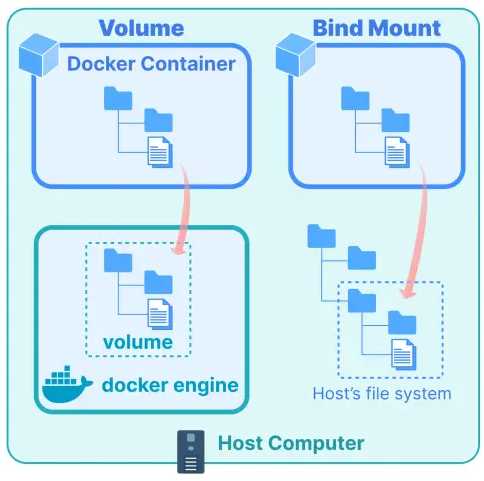
\includegraphics[width=0.48\textwidth]{media/bind-mount}
    \end{center}
\end{frame}

\begin{frame}{Демонстрация: Docker Volumes}
    \textbf{Что покажем:}
    \begin{enumerate}
        \item Работа с bind mounts
        \item Управление docker volumes
    \end{enumerate}

    \vspace{0.2cm}

    \textbf{Демо-репозиторий:} \\
    \href{https://github.com/prafdin/devops-course-demos/tree/docker-additional}{\texttt{https://github.com/prafdin/devops-course-demos/tree/docker-additional}}
\end{frame}

\end{document}